\documentclass{article}
%for the accent
\usepackage[utf8]{inputenc}
%to put an image
\usepackage{graphicx}
\usepackage[french]{babel}
\usepackage[]{amsmath, amsfonts, amssymb, enumerate}
\usepackage{pdfpages} 

%all the things to make a good title
\title{PROJET GENIE LOGICIEL (SINFO015) :\\ Rapport de modélisation}
\author{\textbf{Auteurs}: \\ Adrien Fievet \\ Claire D'Haene \\ Julien Ladeuze \\ Maxime Dupuis}
\date{2022-2023}

\begin{document}

\maketitle

%to skip lines
\vspace{7\baselineskip}

\begin{minipage}{0.4\textwidth}
	\begin{flushleft}
		\large
		\textit{Titulaire}\\
		Tom \textsc{Mens}\\
		\textit{Enseignants}\\
		Sébastien \textsc{Bonte}\\
		Jeremy \textsc{Dubrulle}\\
		Pierre \textsc{Hauweele}	
	\end{flushleft}
\end{minipage}
~
\begin{minipage}{0.5\textwidth}
	\begin{flushright}
		\large
		\textit{Equipe 7}\\
		Adrien (220625) extension\\
		Claire (220323) extension\\
		Julien (220101) extension\\
		Maxime (matricule) extension\\
	\end{flushright}
\end{minipage}

%insert the image
\begin{figure}
    \centering
    
\includegraphics[width = 0.3\textwidth]{images/umons.jpeg}
    \hspace{5em}
    
\includegraphics[width = 0.3\textwidth]{images/facSciences.png}
\end{figure}

%hide the number of the actual page just for the cover page
\thispagestyle{empty}


\newpage
\tableofcontents
\newpage

\subsection{Use cases diagrams}

\begin{flushleft}
Concernant les Use cases pour cette extension, j'ai dû en rajouter deux.
\end{flushleft}

\begin{flushleft}
\textbf{Comparer les données de consommations}, celui-ci va permettre à l'utilisateur comme son nom l'indique de comparer ses données, cette faculté a déjà été expliquée dans l'introduction.
\end{flushleft}

\begin{flushleft}
\textbf{Envoyer un mail}, quant à celui-ci, il spécifie que si une donnée d'un client est anormalement élevée, alors le serveur enverra un mail pour l'avertir, comme expliqué également dans l'introduction.
\end{flushleft}

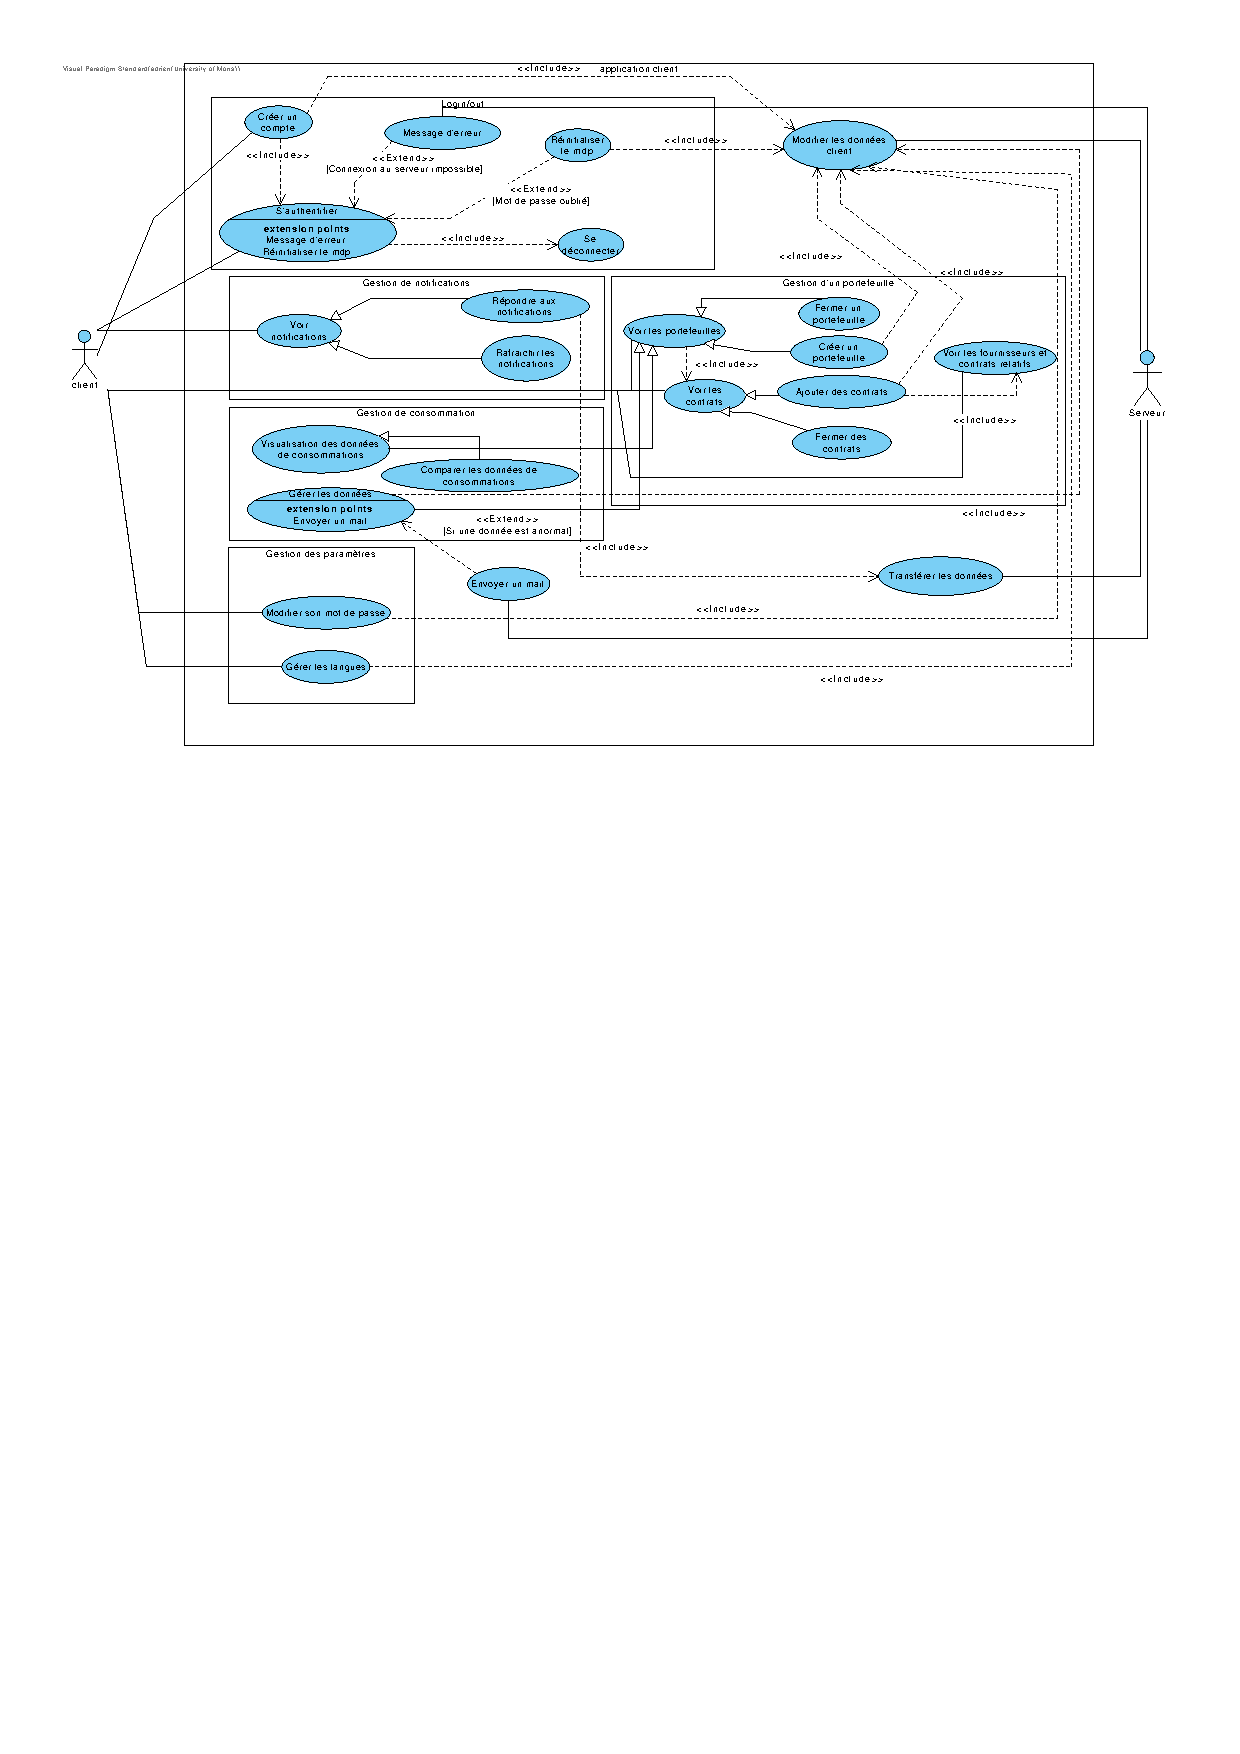
\includepdf[pages=-]{extension_adrien/use_case/img/use_case.pdf}

\subsection{Overview}

\begin{flushleft}
Au niveau de l'overview, j'ai donc ajouter un "interaction use" après la \textbf{Visualisation des données de consommation} car l'utilisateur peut décider de comparer ses données une fois qu'il est dans la visualisation s'il le souhaite.
\end{flushleft}

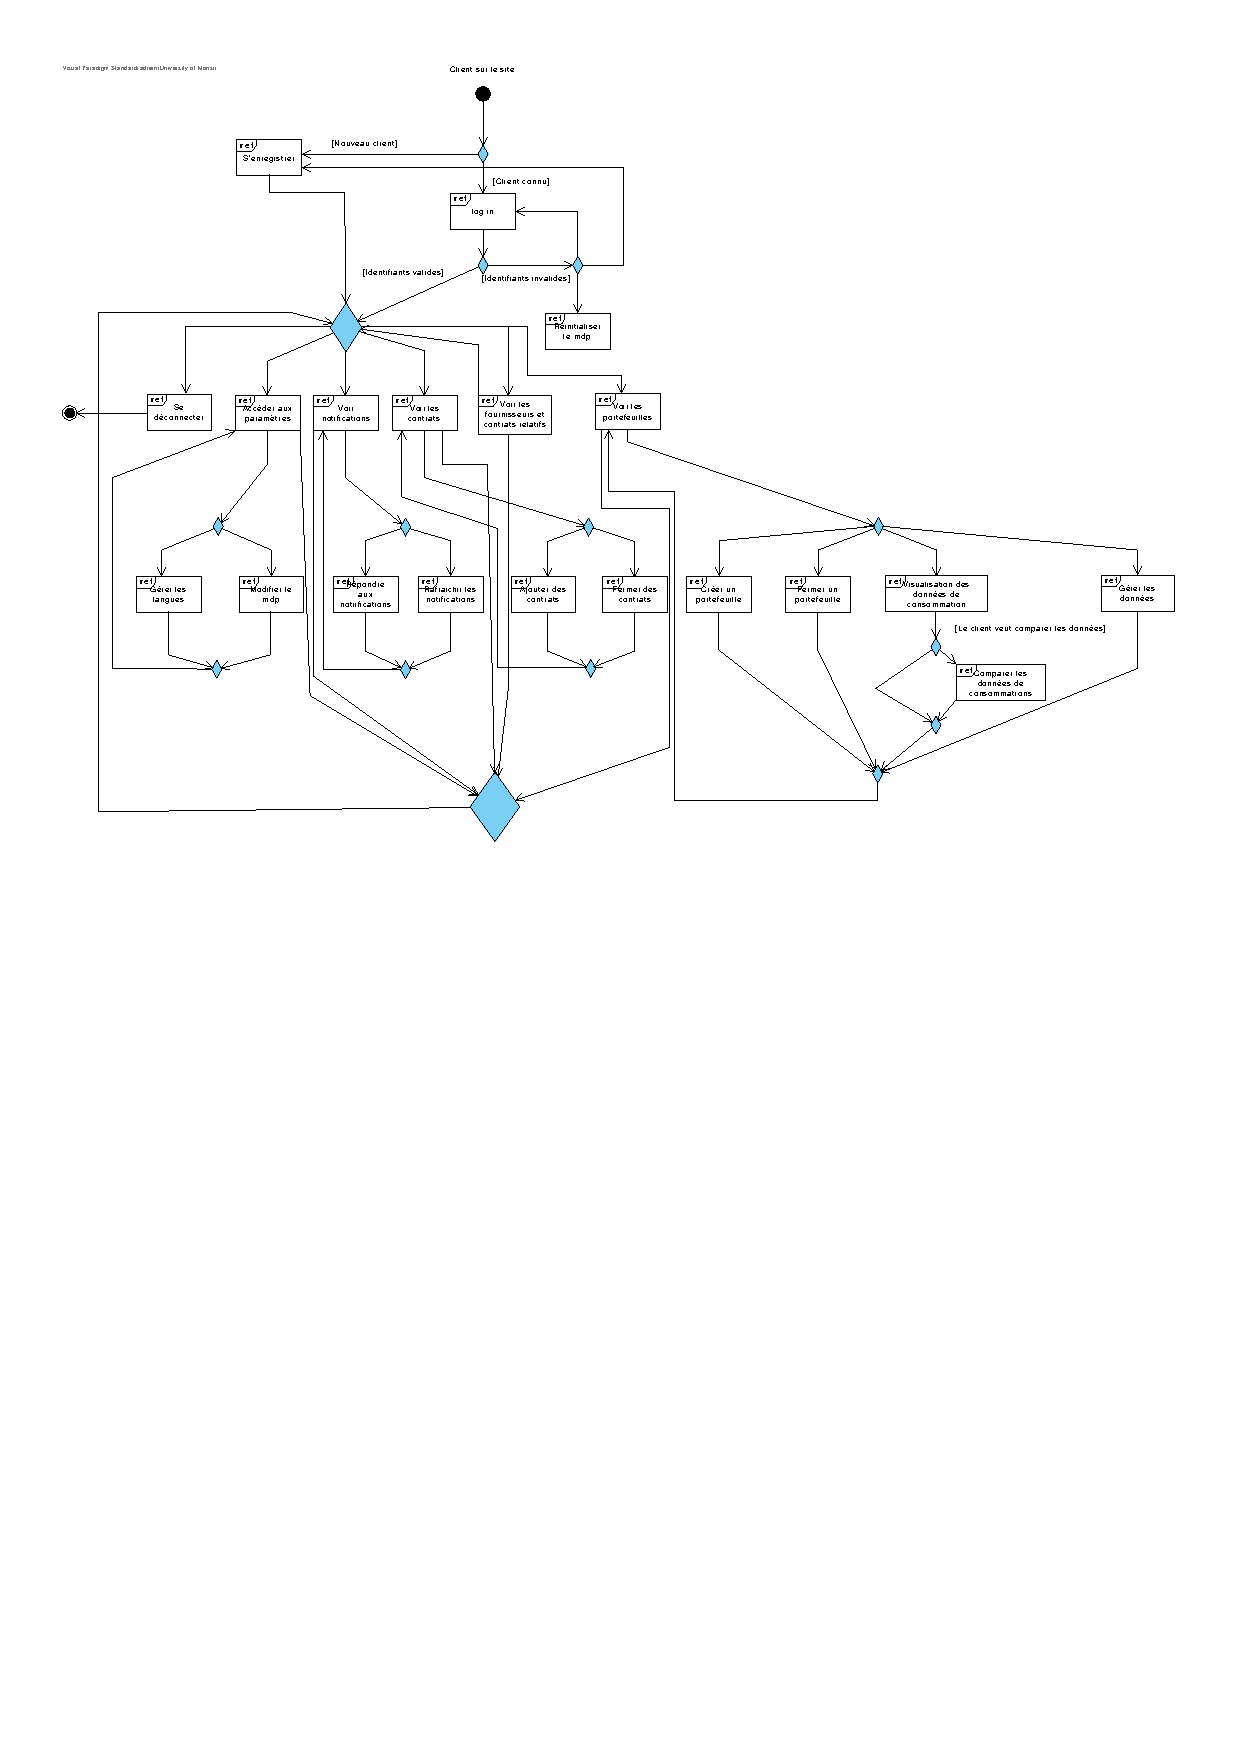
\includepdf[pages=-]{extension_adrien/overview/img/overview.pdf}

\subsection{Interface}

\begin{flushleft}
Pour inclure l'extension dans l'interface, j'ai dû changer 3 pages.
\end{flushleft}

\begin{enumerate}[-]
\item Add a wallet
\item Name (wallet)
\item Consumptions
\end{enumerate}

\begin{flushleft}
Suivant les explications de la base de données, le client devra entrer plus d'informations dans la fenêtre \textbf{Add a wallet} et nous pouvons également les afficher dans \textbf{Name (wallet)} vu que le client souhaite voir toutes les informations du portefeuille dans celui-ci.
\end{flushleft}

\begin{flushleft}
Dans le cas de \textbf{Consumptions}, j'ai d'abord rajouté trois boutons dans le bas de page. Ils représentent les différents modes, c'est-à-dire:
\end{flushleft}

\begin{enumerate}[-]
\item Voir sa consommation \textbf{Just see}
\item Comparer ses consommations \textbf{Compare}
\item Comparer sa consommation avec quelqu'un d'autre (simulation) \textbf{Compare with other}
\end{enumerate}

\begin{flushleft}
Finalement, j'ai placé un tableau en plus pour le cas où l'on veut comparer des données. Comme vous pouvez le voir, il y a également deux boutons au-dessus de chaque tableau qui permettent de choisir si l'on veut voir les données pures ou les statistiques.
\end{flushleft}

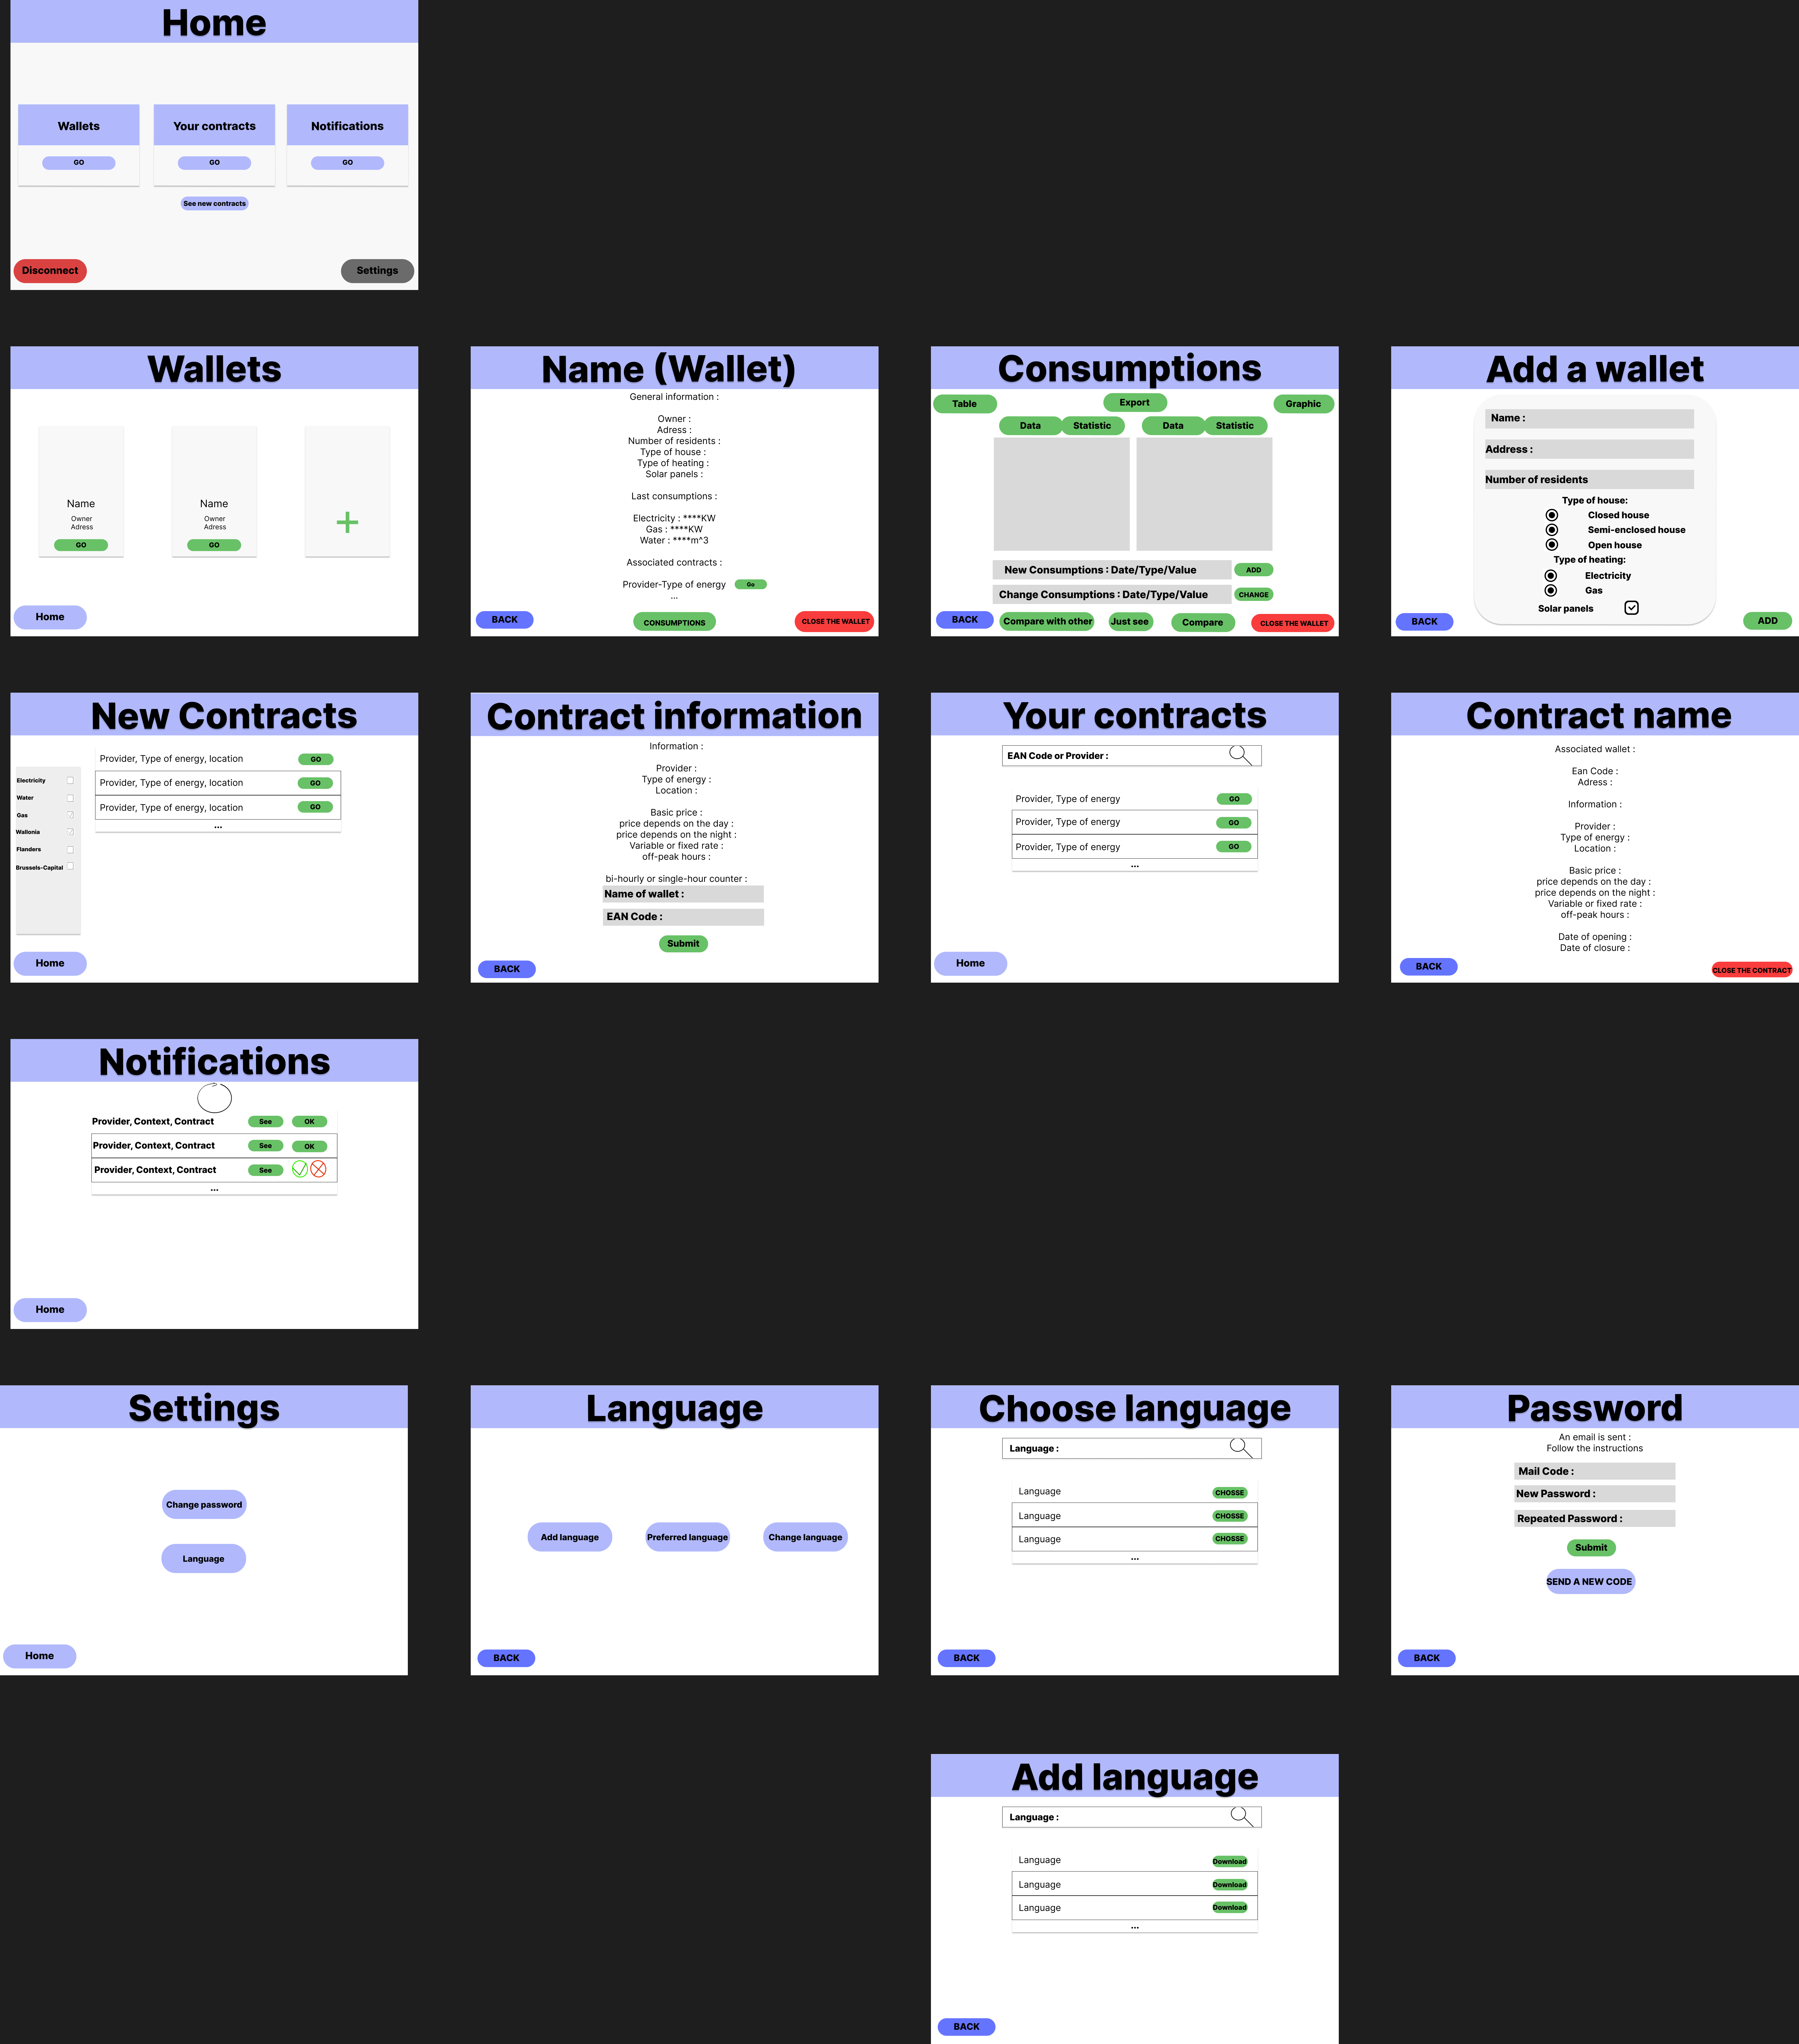
\includepdf[pages=-]{extension_adrien/Interface/img/interface.pdf}


\end{document}
